\documentclass[
  11pt,
  letterpaper,
   addpoints,
   answers
  ]{exam}

\usepackage{../exercise-preamble}
\usepackage{float}

\begin{document}

\noindent
\begin{minipage}{0.47\textwidth}

\includegraphics[width=\textwidth]{../fcfm_die}
\end{minipage}
\begin{minipage}{0.53\textwidth}
\begin{center} 
\large\textbf{Circuitos Eléctricos Analógicos} (EL3202-1) \\
\large\textbf{Clase auxiliar 2} \\
\normalsize Prof.~ Patricio Mendoza.\\
\normalsize Prof.~Aux.~Renato Planas ~Erik Sáez
\end{center}
\end{minipage}

\vspace{0.5cm}
\noindent
\vspace{.85cm}

\begin{questions}
    \question Preguntas teoricas.
\begin{parts}
    \part Explique qué son las impurezas donadoras y las impurezas aceptoras.
    \part ¿A qué es igual el producto de $n_0$ y $p_0$?
    \part ¿De dónde provienen los huecos y electrones en un semiconductor para el caso intrínseco?
    \part Explique cómo se mueve la posición de la Energía de Fermi según se dope un semiconductor con átomos aceptores o átomos donadores.
    \part ¿Qué es la corriente de difusión? ¿Por qué esta corriente es $0$ si se dopa uniformemente un semiconductor?
\end{parts}

\begin{solution}
\subsection*{Resolución 1.1}
Las impurezas son átomos que se añaden a la red cristalina del semiconductor. Recordemos que los semiconductores tienen como material base (normalmente) silicio o germanio, que son átomos pertenecientes al grupo IV de la tabla periódica (4 electrones de valencia). Con esto en mente, las impurezas donadoras son aquellos átomos del grupo V que se agregan a la red cristalina, estos tienen 5 electrones de valencia, por lo que al integrarse a la red, considerando que en el enlace atómico se tiene a cumplir la regla del octeto, queda un electrón libre circulando. Para esto principalmente se utiliza el fósforo como material donante. Las impurezas donadoras son aquellos átomos del grupo III (normalmente boro) y al tener 3 electrones de valencia queda un hueco libre.

\subsection*{Resolución 1.2}
Bajo ciertas condiciones (temperatura suficiente, masa efectiva considerable, entre otros supuestos de la mecánica estadística) se puede definir la ley de acción de masas con la siguiente ecuación:
$$n_0 p_0 = n_i^2$$

Donde $n_0$ es la concentración de electrones en la banda de conducción, $p_0$ la concentración de huecos en la banda de valencia y $n_i$ la concentración intrínseca de portadores de carga. Esta ecuación es válida tanto para materiales (intrínsecos) o dopados.

\textbf{Aproximaciones:} Si se tiene un material tipo N (dopado con impurezas donadoras) el número de electrones será mayor que el número de huecos y se puede aproximar $n_0 = N_d$, donde $N_d$ es la concentración de impurezas donadoras.

De igual forma, en el caso de tipo P, se puede aproximar $p_0 = N_a$. Para que lo anterior sea importante que la temperatura sea suficiente para que todas las impurezas sean ionizadas.

Además, para que ambas aproximaciones sean válidas, la concentración de portadores intrínsecos debe ser considerablemente menor a la concentración de átomos donantes/aceptores.

\subsection*{Resolución 1.3}
En un semiconductor intrínseco se generan pares hueco-electrón gracias a la acción de la temperatura. A medida que aumenta la temperatura, la energía térmica dada por $kT$ (donde $k$ es la constante de Boltzmann) aumenta y con ello se rompen enlaces en la red cristalina. Al romperse un enlace el electrón participante puede movilizarse por la red (electrón) mientras que en el enlace roto queda un espacio disponible para enlazarse (hueco).

\subsection*{Resolución 1.4}
En la definición más simple, la energía de Fermi es el nivel de energía bajo el cual todos los estados cuánticos están utilizados con electrones y por encima están todos los estados vacíos, a $0$ K. Una primera buena interpretación de esta definición puede ser ver la posición de la energía de Fermi y con eso concluir acerca de la concentración de electrones y huecos en el semiconductor: En el caso intrínseco la energía de Fermi está en medio de la posición de la banda de valencia y de conducción. En el caso de tipo N, la energía de Fermi se mueve hacia la banda de conducción (sube) y en el tipo P la energía de Fermi se desplaza hacia la banda de valencia (baja).

\subsection*{Resolución 1.5}
La corriente de difusión es la corriente que se genera en un semiconductor debido al flujo de partículas cargadas desde una región de alta concentración hacia una región de baja concentración. 

$$J_n = e D_n \frac{dn}{dx} \quad \text{y como también la concentración,}$$

$$\text{Corriente del electrón}$$

Para huecos es análogo:
$$J_p = -e D_p \frac{dp}{dx}$$

Si se dopa uniformemente un semiconductor, no hay gradiente de concentración ($\frac{dn}{dx} = 0$ y $\frac{dp}{dx} = 0$), por lo que la corriente de difusión es cero.
\end{solution}

%------
\question
Calcule las concentraciones de huecos y electrones en un material semiconductor de silicio que tiene una concentración intrínseca de $n_i = 10^{10}\,\text{cm}^{-3}$, cuando este material se encuentra a una temperatura de $293^\circ \text{K}$. Explicite en qué banda de energía se encuentra respectivamente cada tipo de partícula (hueco o electrón).

\question
Un material semiconductor está formado principalmente de silicio, con concentración intrínseca de $n_i = 10^{10}\,\text{cm}^{-3}$, pero dopado con partículas de fósforo con una concentración de $10^{17}\,\text{cm}^{-3}$. Cuando este material se encuentra a una temperatura de $293^\circ \text{K}$:
\begin{parts}
    \part Calcule las concentraciones de huecos y electrones utilizando el método exacto.
    \part Calcule las concentraciones de huecos y electrones utilizando el método aproximado.
    \part ¿Cuál es el error cometido al aproximar? ¿Qué ecuación no se cumple al hacer la aproximación?
    \part Explicite en qué banda de energía se encuentran respectivamente cada tipo de partícula (hueco o electrón).
    \part ¿Qué tipo de material es este semiconductor?
\end{parts}

\question
Un material semiconductor está formado principalmente de silicio pero que ha sido dopado en una parte con moléculas de Boro (parte gris de la Figura \ref{fig:p3}) con una concentración de $10^{16}\,\text{cm}^{-3}$ y dopado con partículas de fósforo con una concentración de $10^{17}\,\text{cm}^{-3}$ (parte blanca de la Figura \ref{fig:p3}). Recuerde que el silicio tiene una concentración intrínseca de $n_i = 10^{10}\,\text{cm}^{-3}$ cuando este material se encuentra operando a una temperatura de $293^\circ \text{K}$.

\begin{parts}
    \part ¿Qué tipo de materiales son cada parte dopada diferente?
    \part ¿Cuáles son las concentraciones de equilibrio en este material?
    \part ¿Existe un voltaje entre los dos tipos de materiales? Si es así, ¿cuál es el valor?
    \part ¿Qué representan las curvas verdes y azules en la Figura?, ¿qué representan la Abscisa y la Ordenada en la figura?
    \part Bosqueje un diagrama de bandas de energía para esta situación.
\end{parts}

\begin{figure}[H]
    \centering
    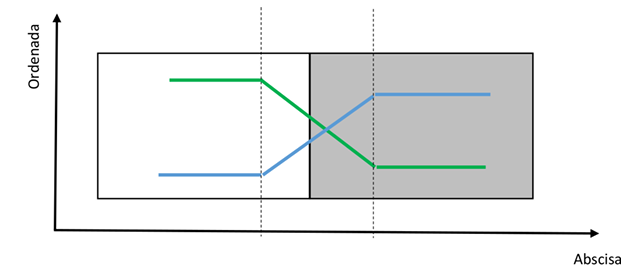
\includegraphics[width=0.7\textwidth]{../figures/Auxiliar_2_1}
    \caption{Problema 3}
    \label{fig:p3}
\end{figure}

\question
Para el mismo material del problema 3 ahora se ve que en la curva verde existe un cambio como se nota en la Figura \ref{fig:p4}:

\begin{parts}
    \part ¿Qué pudo haber producido este cambio?
    \part Si conociera el valor del punto rojo, ¿podría estimar el valor de la variable que está produciendo el cambio?
    \part ¿Qué necesitaría conocer para estimar la densidad de corriente asociada a esta curva? ¿Cuál sería su expresión si tuviera conocido todo lo que requiere?
    \part Bosqueje un diagrama de energía para esta situación.
\end{parts}

\begin{figure}[H]
    \centering
    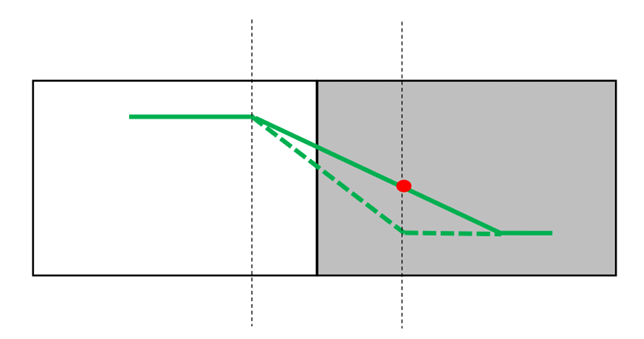
\includegraphics[width=0.7\textwidth]{../figures/Auxiliar_2_2}
    \caption{Problema 4}
    \label{fig:p4}
\end{figure}

\end{questions}

\end{document}